\section{Objectives}

Following handout PDF pages 115--118, compare full and reduced single-phase latches, double N/P clocked inverters, and two-stage DFF chains with full/reduced first stages. An additional mid-phase input-change test addresses the requested limitations.

\section{Handout requirements and test mapping}

\begin{center}
\small
\setlength{\tabcolsep}{4pt}
\begin{tabular}{p{.42\linewidth}p{.29\linewidth}p{.18\linewidth}}
\toprule
Requirement & Deck prefix and conditions & Status \\
\midrule
Step 1: Fig. 28.1 a/c and b/d comparisons & 01; independent copies & Waveforms and differences measured \\
Step 2: double N/P inverter hold & 02; data changes while held & Hold windows measured \\
Q1: P/N-latch DFF, cascade two & 03; 0.2/1 ns clock edges & Periodic data measured \\
Q2: remove first stage; limits/internal nodes & 03/04; periodic and hazard data & Counterexample retained \\
\bottomrule
\end{tabular}
\end{center}

\section{Topology and expected behavior}

The second stage in Fig. 28.1(a)/(b) is a full clocked inverter. Versions (c)/(d) remove the complementary-clock device that is redundant for the corresponding dynamic-node state. The full DFF combines P then N sections, giving four inversions. Removing the first stage leaves three inversions, reversing single-stage output polarity. Cascade expectations must account for this parity; first-stage waveforms cannot simply be subtracted point by point.

A single-phase architecture removes the external two-phase clock requirement but does not make internal nodes static memories. A dynamic precharge/evaluate node may support only one transition direction, and full versus reduced structures need not tolerate the same within-phase input changes.

\section{Simulation setup and interpretation}

The supplied encrypted MOS model is evaluated at a baseline supply of 1.0 V and 25\,$^\circ$C. The 1.0 V value is a teaching condition, not a verified voltage rating. These results do not reproduce the handout's original process or supply conditions. Unless stated in the deck, $W_n/W_p/L=0.6/1.8/0.25\,\mu\mathrm m$, bulks are tied to their corresponding rails, and output load is 5 fF. Transmission-gate and weak-feedback dimensions are specified explicitly in each deck.

PrimeSim HSPICE S-2021.09 win64 was used with \texttt{RUNLVL=6}, \texttt{ACCURATE}, and \texttt{WARNLIMIT=100}. Every baseline and \texttt{.alter} analysis concluded without errors or failed measurements. The simulator still reports suppressed warnings associated with encrypted blocks; this does not establish that the model is warning-free or that those warnings are harmless. The \texttt{.tran} print interval is not a fixed integration step: the solver uses adaptive timesteps. A finite sweep is not a complete process qualification.

Unless stated otherwise, the declared functional diagnostic uses $V\leq0.2$ V for low and $V\geq0.8$ V for high. These are report-level interpretation thresholds, not numerical handout requirements or extracted receiver noise margins. Correct samples do not exclude glitches between samples. Figures are redrawn from actual simulation data; \texttt{results/} contains per-case waveforms, measurements, and derived comparison CSV files.

Public decks omit model loading paths; model configuration is added only to local execution copies. The model itself is not distributed. The first two filename digits identify the deck numbers used below. Every deck is standalone.

\section{Results}

\begin{center}
\small
\setlength{\tabcolsep}{4pt}
\begin{tabular}{lr}
\toprule
Pair & Maximum sampled voltage difference (V) \\
\midrule
1-3 & 0.174150 \\
2-4 & 0.043550 \\
\bottomrule
\end{tabular}
\end{center}

\begin{figure}[htbp]
\centering
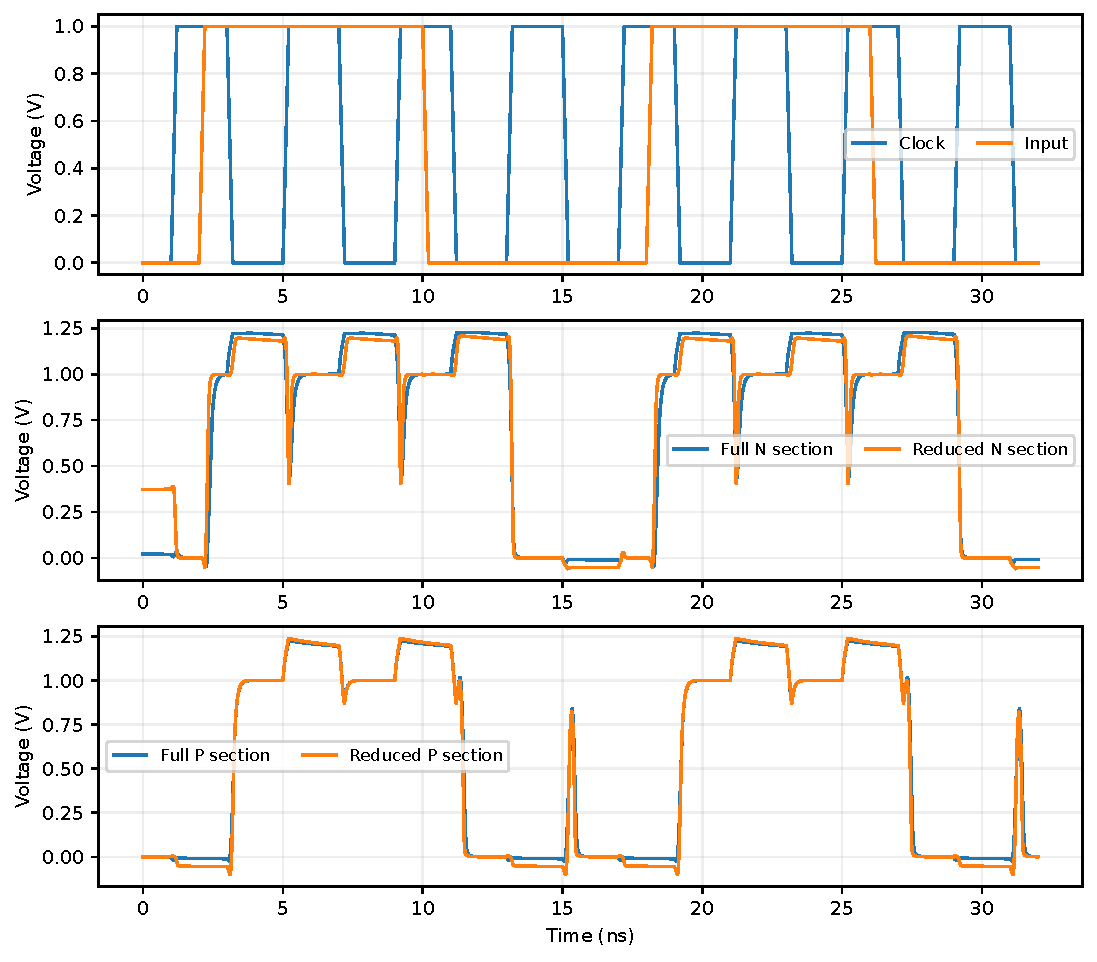
\includegraphics[width=.96\linewidth]{figures/latch_equivalence.pdf}
\caption{Paired full and simplified latches; matching logic does not mean identical analog waveforms.}
\end{figure}

Paired logic agrees at the six sample times, while maximum N-section difference is 0.174150 V and P-section difference 0.043550 V. Some highs exceed 1 V and lows dip below 0 V because of floating nodes and clock feedthrough. These values must not be clipped to ideal 0/1 before claiming equivalence.

\begin{center}
\small
\setlength{\tabcolsep}{4pt}
\begin{tabular}{lrrr}
\toprule
Double inverter & Hold minimum (V) & Maximum (V) & Span (V) \\
\midrule
n & -0.052238 & -0.038262 & 0.013977 \\
p & 1.185680 & 1.214528 & 0.028848 \\
\bottomrule
\end{tabular}
\end{center}

\begin{figure}[htbp]
\centering
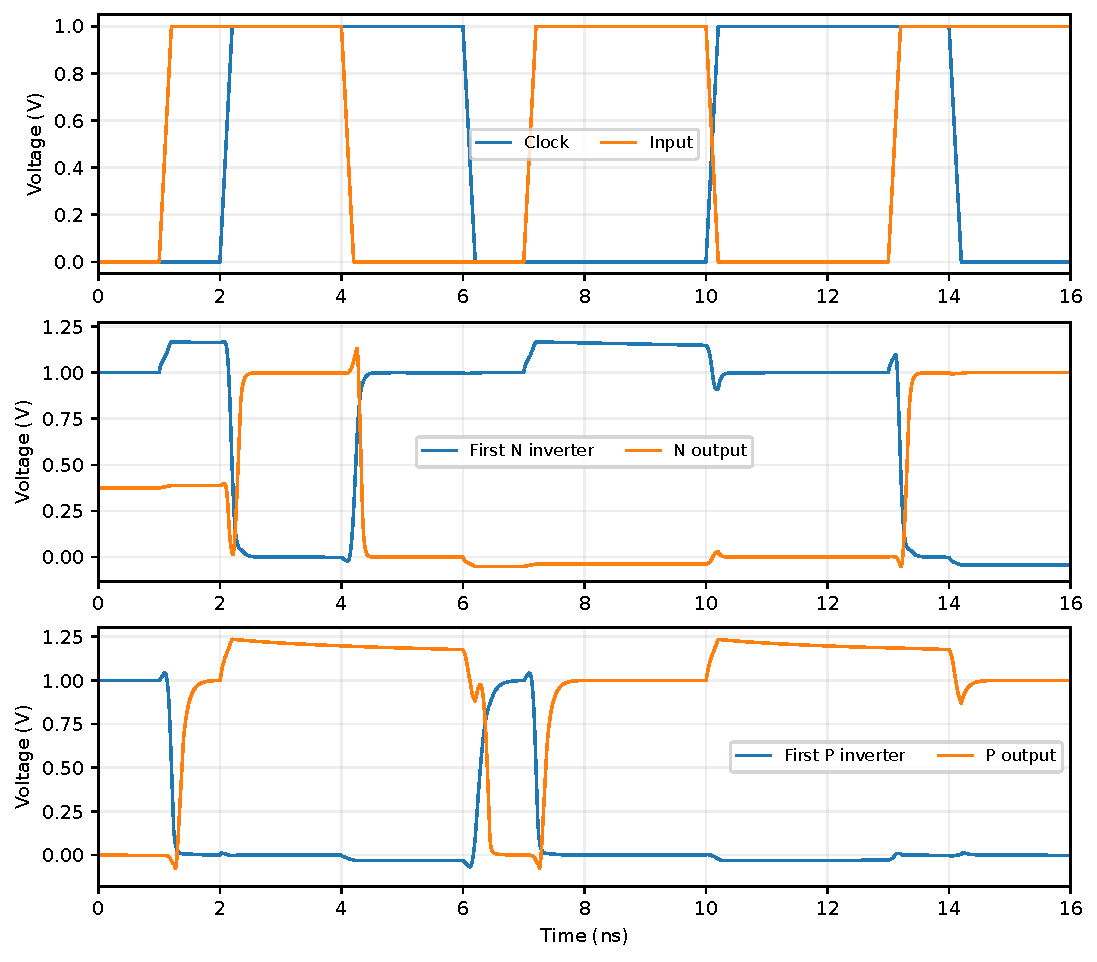
\includegraphics[width=.96\linewidth]{figures/doubled_inverters.pdf}
\caption{Input changes inside the selected hold windows: 7--9 ns for the N pair and 3--5 ns for the P pair.}
\end{figure}

The N pair holds low and the P pair high, but analog levels are approximately -0.05 V and 1.2 V. Holding the intended logic and remaining at ideal supply rails are distinct properties.

\begin{center}
\small
\setlength{\tabcolsep}{4pt}
\begin{tabular}{lrr}
\toprule
Clock edge (ns) & Output & Correct samples/6 \\
\midrule
0.2 & f1 & 6 \\
0.2 & f2 & 6 \\
0.2 & s1 & 6 \\
0.2 & s2 & 6 \\
1 & f1 & 6 \\
1 & f2 & 6 \\
1 & s1 & 6 \\
1 & s2 & 6 \\
\bottomrule
\end{tabular}
\end{center}

\begin{figure}[htbp]
\centering
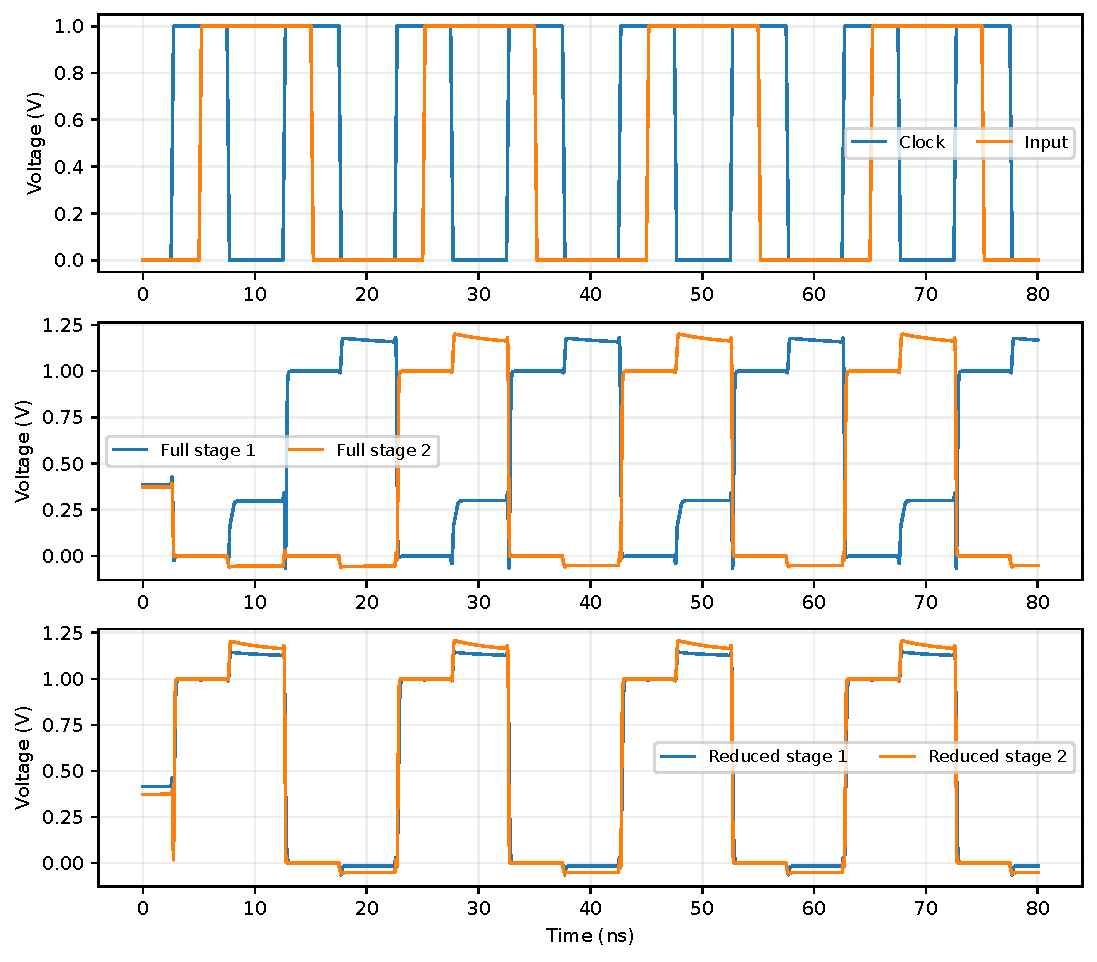
\includegraphics[width=.96\linewidth]{figures/cascade.pdf}
\caption{Two full/reduced DFF stages under periodic data; first-stage polarity differs.}
\end{figure}

With both 0.2 ns and 1 ns clock edges, all four outputs give 6/6 correct selected samples. This periodic input changes during the high phase and is settled before the next low phase begins; it does not prove acceptance of arbitrary within-phase changes.

\subsection{Limitation test and internal nodes}

\begin{figure}[htbp]
\centering
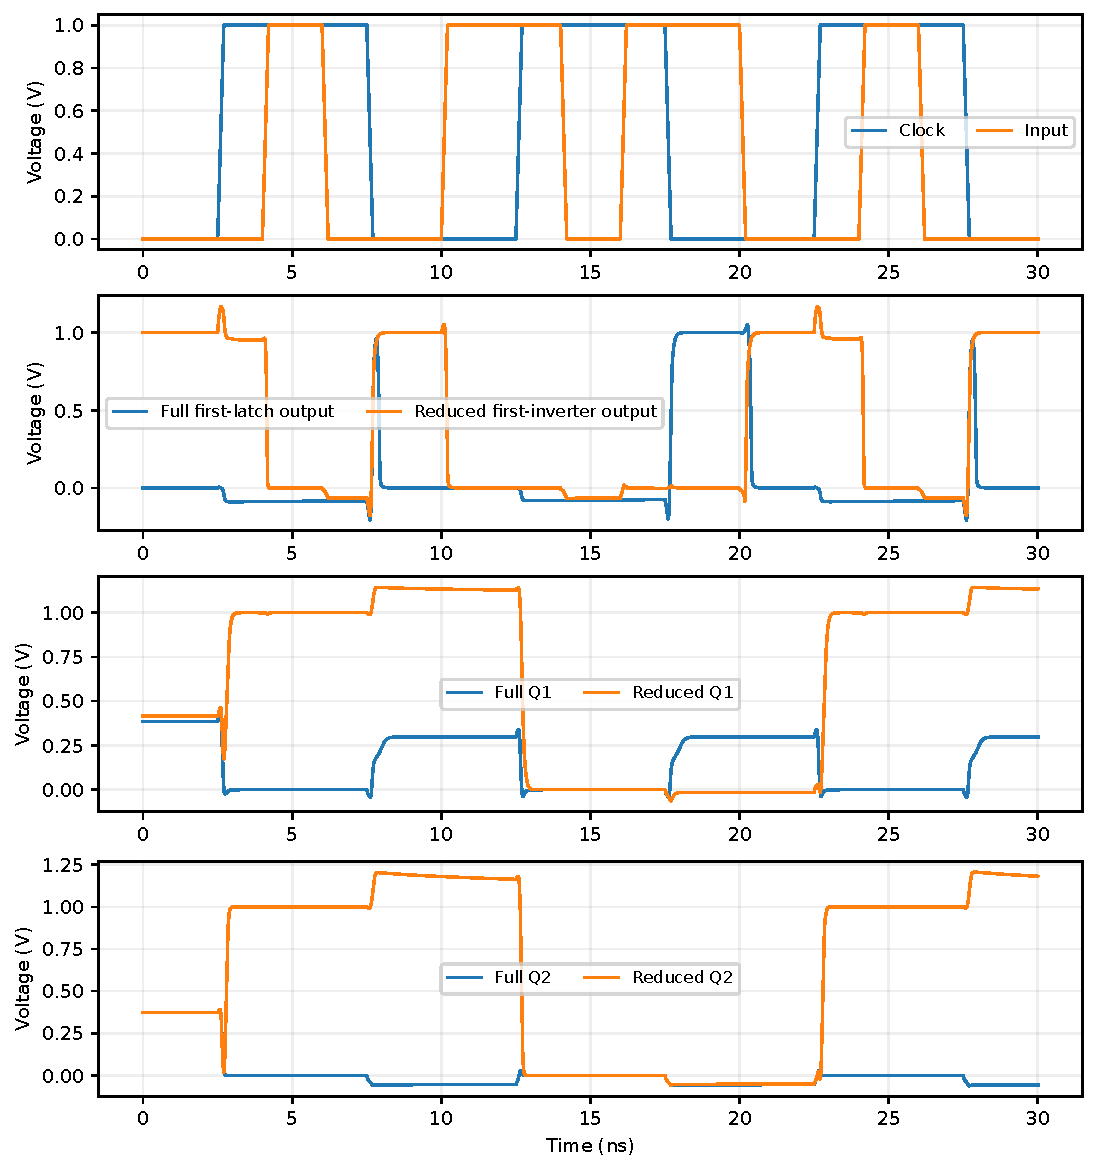
\includegraphics[width=.96\linewidth]{figures/input_timing_limit.pdf}
\caption{Additional data-timing test: the full dynamic P first stage retains previously evaluated charge, while the reduced circuit holds internal state differently.}
\end{figure}

The clock begins rising at 2.5, 12.5, and 22.5 ns. During the first high phase, input rises from 0 to 1 and returns to 0. The reduced internal node moves from 0.953449 to -0.063530 V while output remains approximately 0.999933 V: the internal node is not a complete static hold, yet completed evaluation can preserve the output. The full first-latch output moves from -0.087237 to -0.081927 V over the same interval.

In the second cycle, input changes 0 to 1 at 10 ns within the low phase. The full P-dynamic first node was already charged high and has no low-phase discharge path, so the full first-stage output remains near 0 V at 16.8 ns rather than capturing the 1 expected from a general positive-edge DFF. The reduced first stage is also near 0 V, consistent with its inverted output, and the two cascades exhibit different data sequences. This limitation counterexample preserves the handout topology; failing behavior is neither omitted nor hidden by substituting a different static DFF.

\section{Discussion, differences, and unverified scope}

The Q1/Q2 question of correct operation requires explicit data-timing conditions: the periodic test operates, while arbitrary within-phase changes are not unconditionally equivalent to a general DFF. The full P-dynamic first stage is specifically constrained by monotonic evaluation. Although the reduced circuit preserves expected logic in the added test, partially floating internal nodes still impose setup/hold, leakage, and edge-rate limits. Six correct fixed samples are not extended into a guarantee over full hold windows, all initial states, or arbitrary frequency. The Fig. 28.5 labels 26.1(c/d) are interpreted from context as 28.1(c/d).
